%\documentclass[aps,prd,nofootinbib]{revtex4-1}
\documentclass[singlepage,notitlepage,nofootinbib,11pt]{revtex4-1}
\usepackage{amsmath}
\usepackage{graphicx}
\usepackage{subfig}
\usepackage{epsfig}
\usepackage{listings}
\usepackage[hidelinks,hyperfootnotes=false,bookmarks=false,colorlinks=true]{hyperref}
\begin{document}
\title{Problem Set 2 - G6080}
\author{Victor Genty}
\email{vgenty@nevis.columbia.edu}
\homepage{www.nevis.columbia.edu/~vgenty}
%\affiliation{Department of Physics, Duke University, Durham, NC 27707, USA}
\date{\today}
\begin{abstract}
\centering
Source code can be found at \href{https://github.com/vgenty/G6080/tree/master/ps2}{github.com/vgenty/G6080/ps2}
\end{abstract}
\maketitle
\section{Problem 1 - Planets}
\subsection{Part 1}
The lowest order predictor-corrector method is implemented in Python with the NumPy library to evolve the N body equations of motion. Using the initial conditions specified in Part 1, we find that a step size ``\verb|p.dx|'' of roughly $\mathbf{10^{-4}}$ with $\mathbf{300}\text{\bf{,}}\mathbf{000}$ steps was sufficient to keep the energy from deviating either above or below its initial energy by one percent.
\begin{figure}[h]
  \centering
  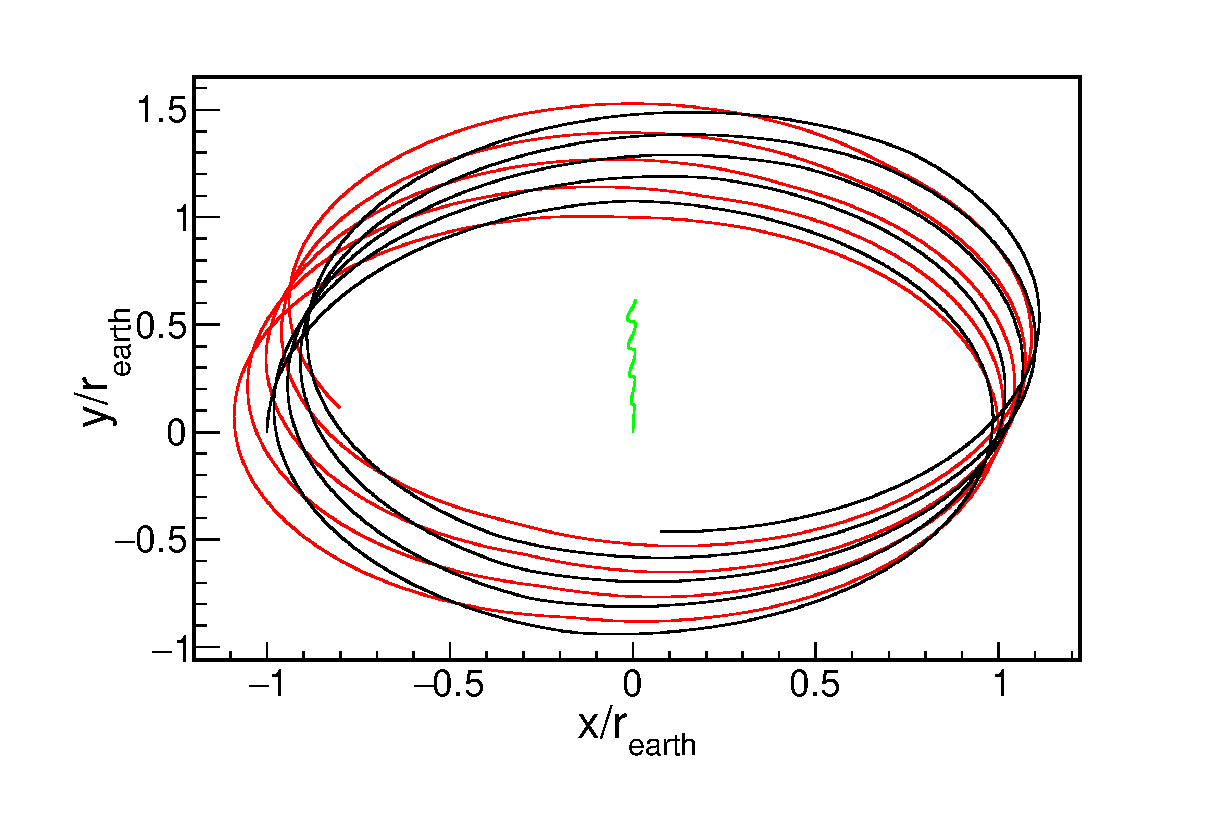
\includegraphics[width=0.5\textwidth]{figures/1r.eps}
  \subfloat[][]{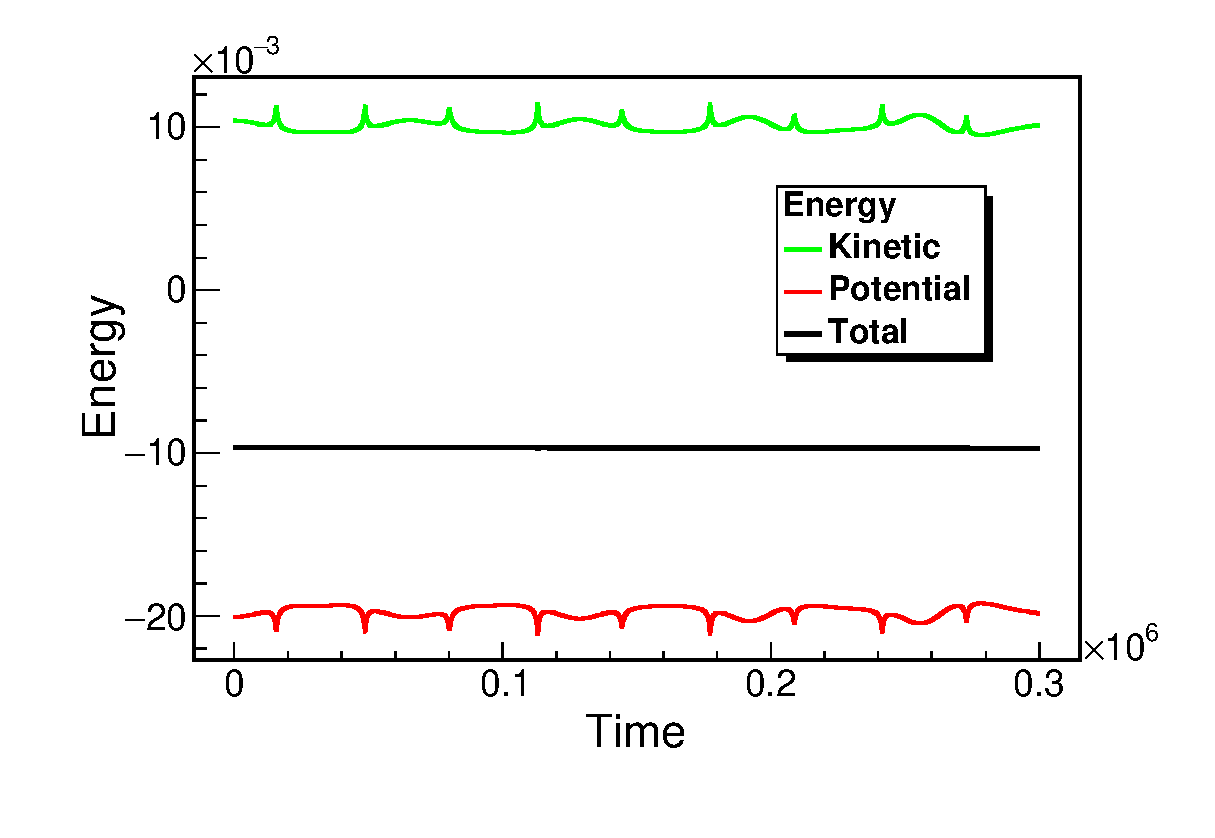
\includegraphics[width=0.5\textwidth]{figures/1es.eps}}
  \subfloat[][]{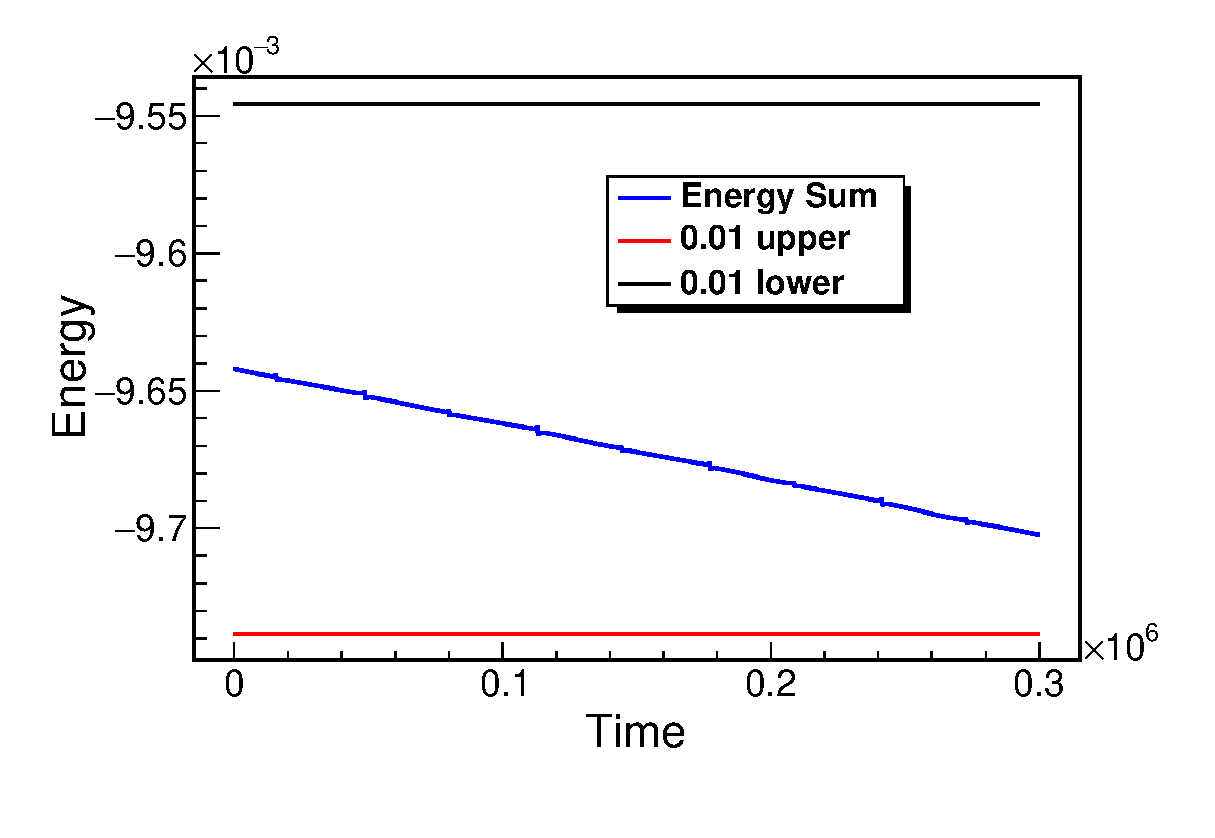
\includegraphics[width=0.5\textwidth]{figures/1ee.eps}}\\
\hfill
  \caption{\label{fig1} Plots for Part 1. Top pane are the coordinate locations of the three planets the green, red, and black lines represent the trajectories of the sun and two orbiting planets. The bottom left pane shows the total kinetic and potential energies. The bottom right shows the deviation of the total energy as a function of time. The lines above and below represent 1\% bounds on the initial total energy.}
\end{figure}
The trajectory, kinetic, potential, and total energy are plotted in Fig. \ref{fig1}.
\clearpage
\subsection{Part 2}
With the initial conditions specified in Part 2 and a step size of 60,000, the predictor-corrector algorithm fails for short range interactions shown in Fig. \ref{fig2}.
\begin{figure}[h]
  \centering
  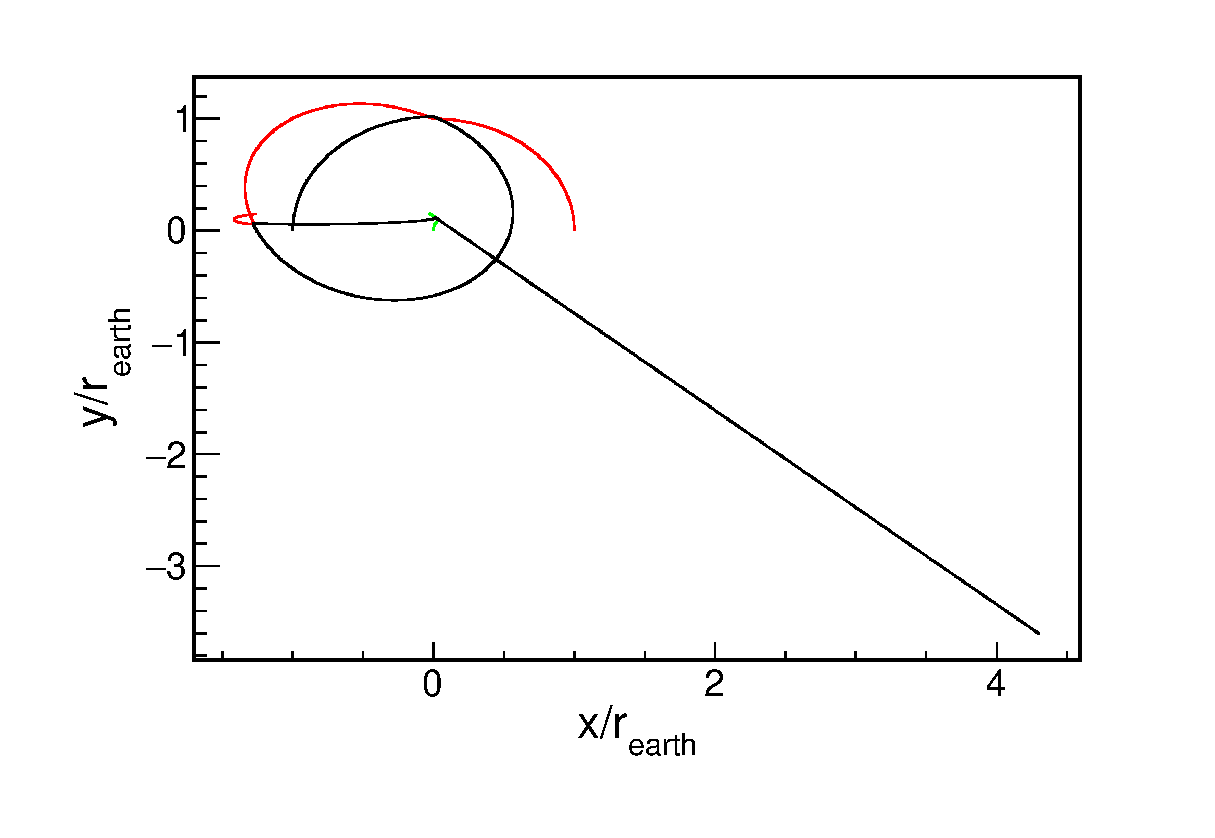
\includegraphics[width=0.5\textwidth]{figures/2r.eps}
  \subfloat[][]{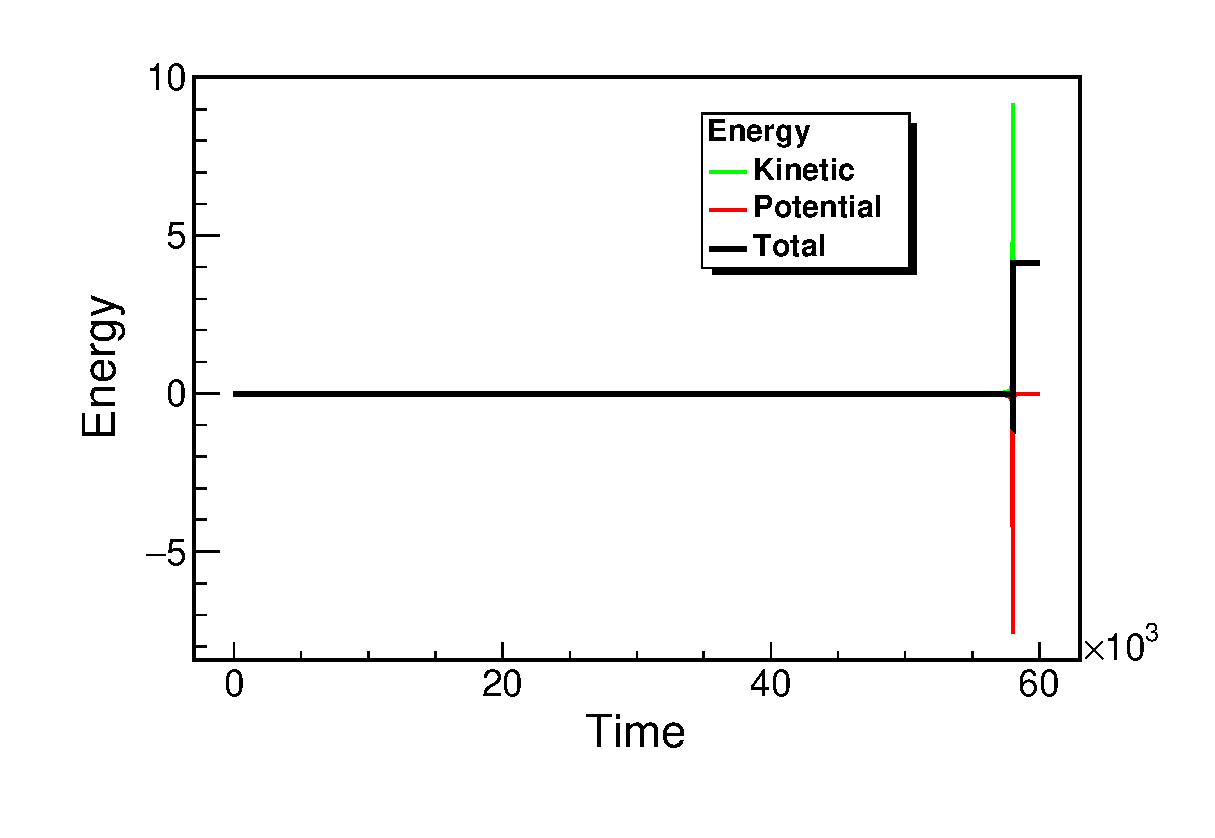
\includegraphics[width=0.5\textwidth]{figures/2es.eps}}
  \subfloat[][]{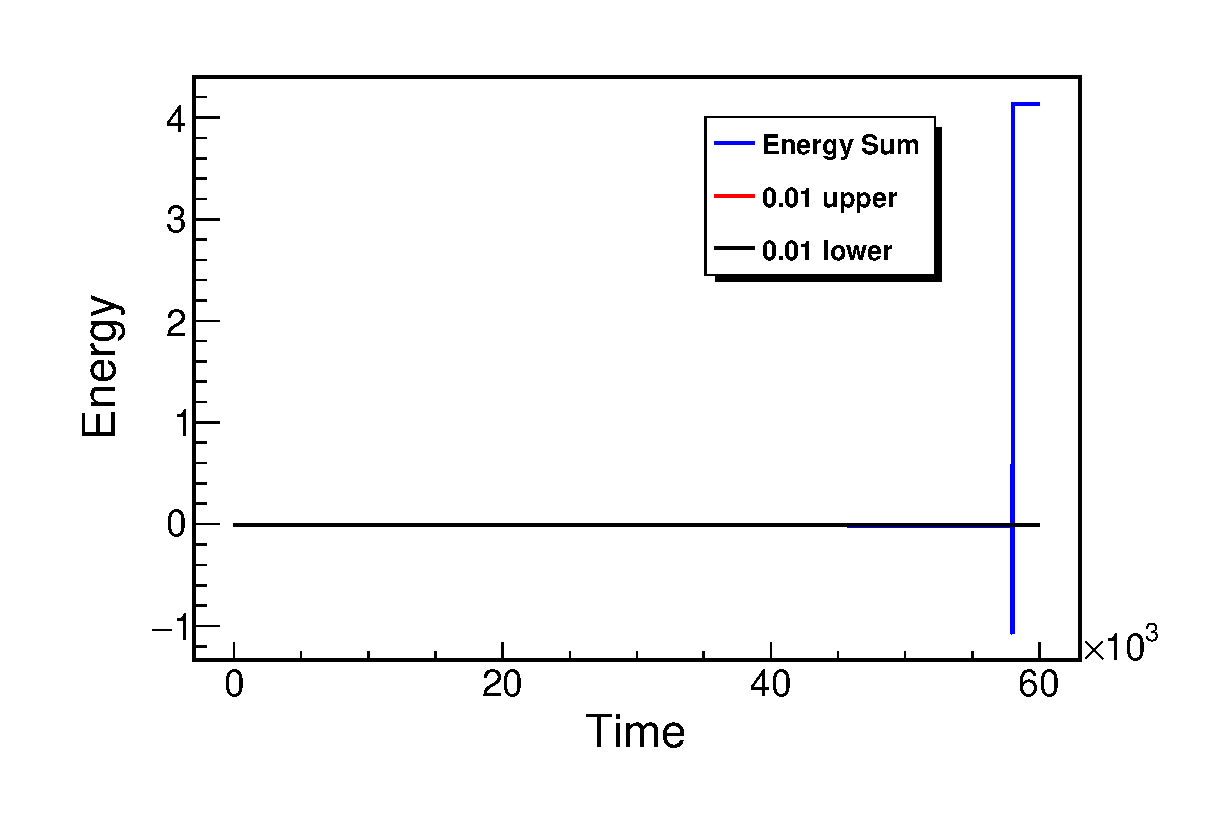
\includegraphics[width=0.5\textwidth]{figures/2ee.eps}}\\
\hfill
  \caption{\label{fig2} Plots for part 2. Top pane shows the three trajectories of the planets. The energy spectrum near the end of the simulation blows up as one of the planet is ejected out of a bound orbit.}
\end{figure}
One of the planets is ejected from an initially bound orbit via two interactions with the second planet, and a fatal interaction with the massive sun. The total energy of the system explodes in the final steps as the step size on the predictor corrector algorithm is too large.
\clearpage
\subsection{Part 3}
In order to see the two planet interactions in the previous part we increase the number of iterations to {\bf 120,000} and decrease the step size to $\mathbf{4.0\times10^{-5}}$. I increased the evolution time past 75,000 as stated in the problem (an increase of 25\%) in order to observe the planets interact twice in their orbits around the sun. Reducing the step size greatly constrained deviation of the total energy. The step size must be much smaller due to the large predicted velocity and force during the close interaction when the potential energy is strongly negative. The results are plotted in Fig. \ref{fig3}
\begin{figure}[h]
  \centering
  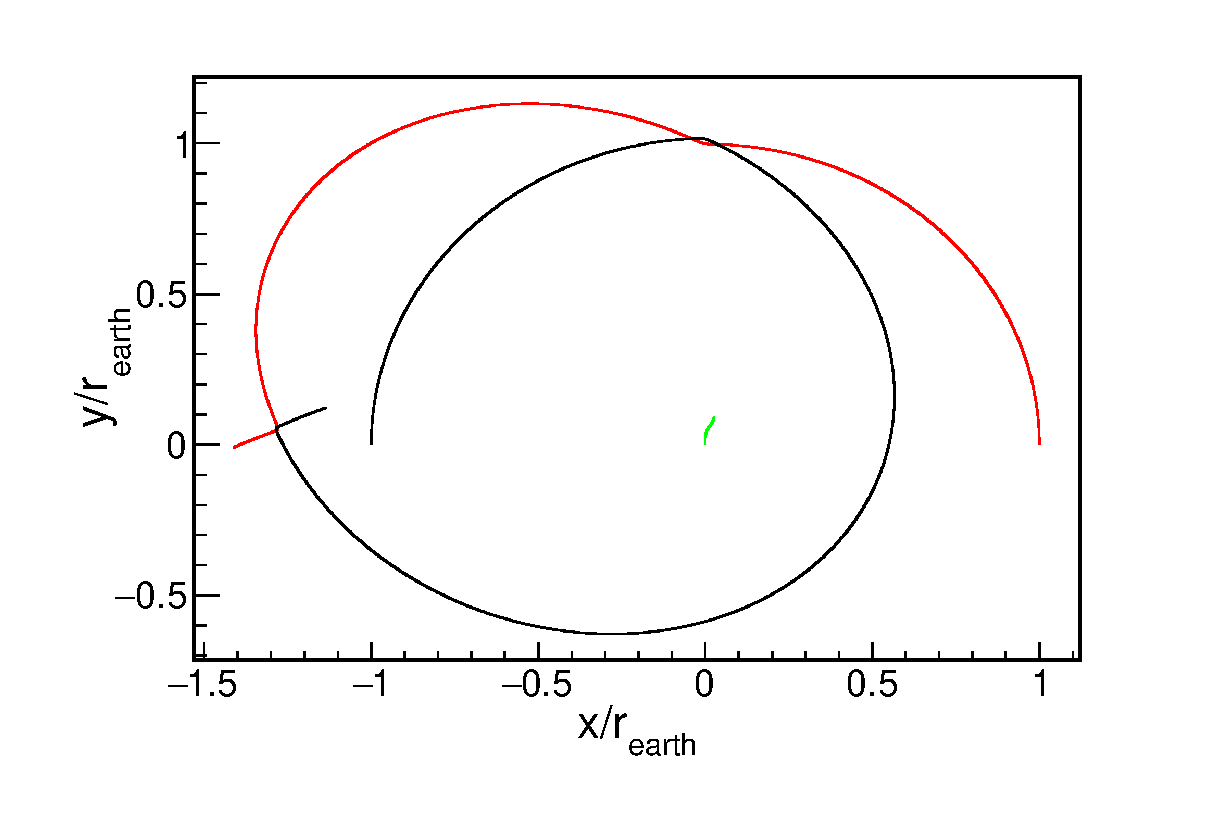
\includegraphics[width=0.5\textwidth]{figures/3r.eps}
  \subfloat[][]{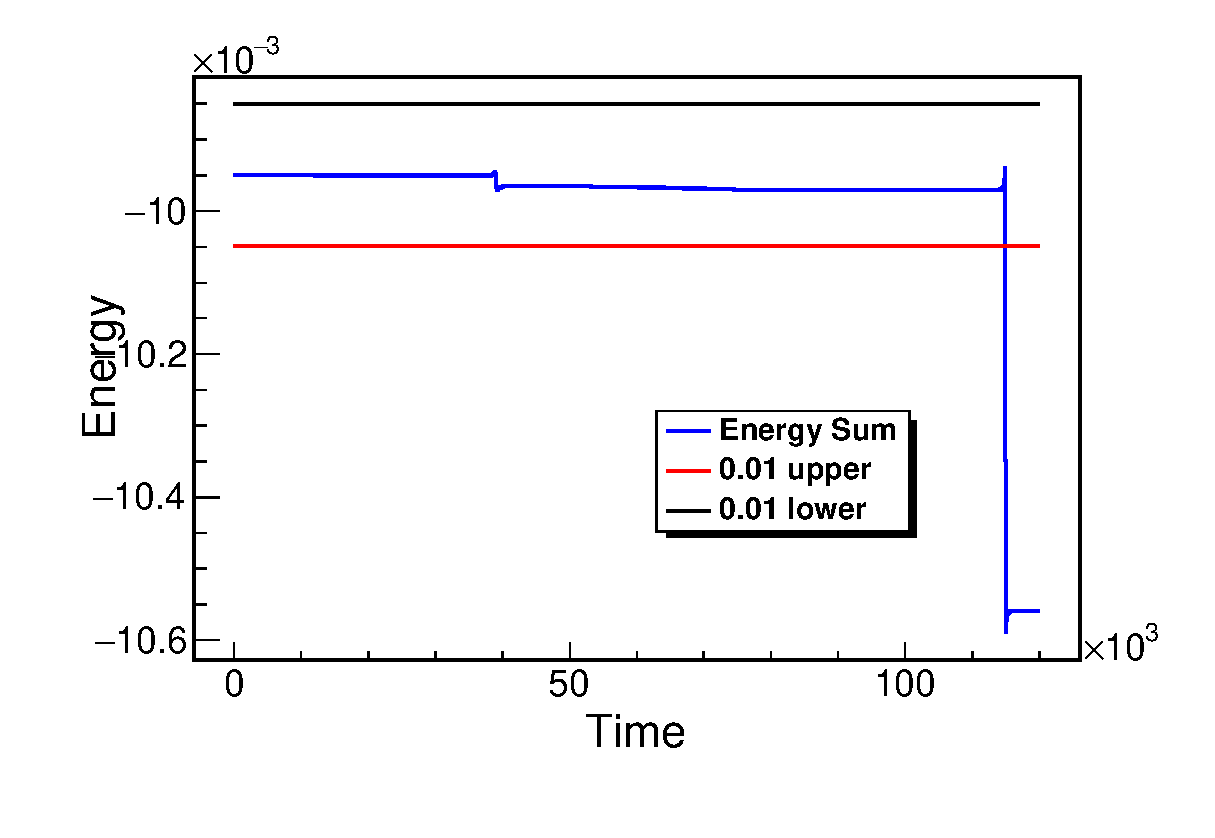
\includegraphics[width=0.5\textwidth]{figures/3es.eps}}
  \subfloat[][]{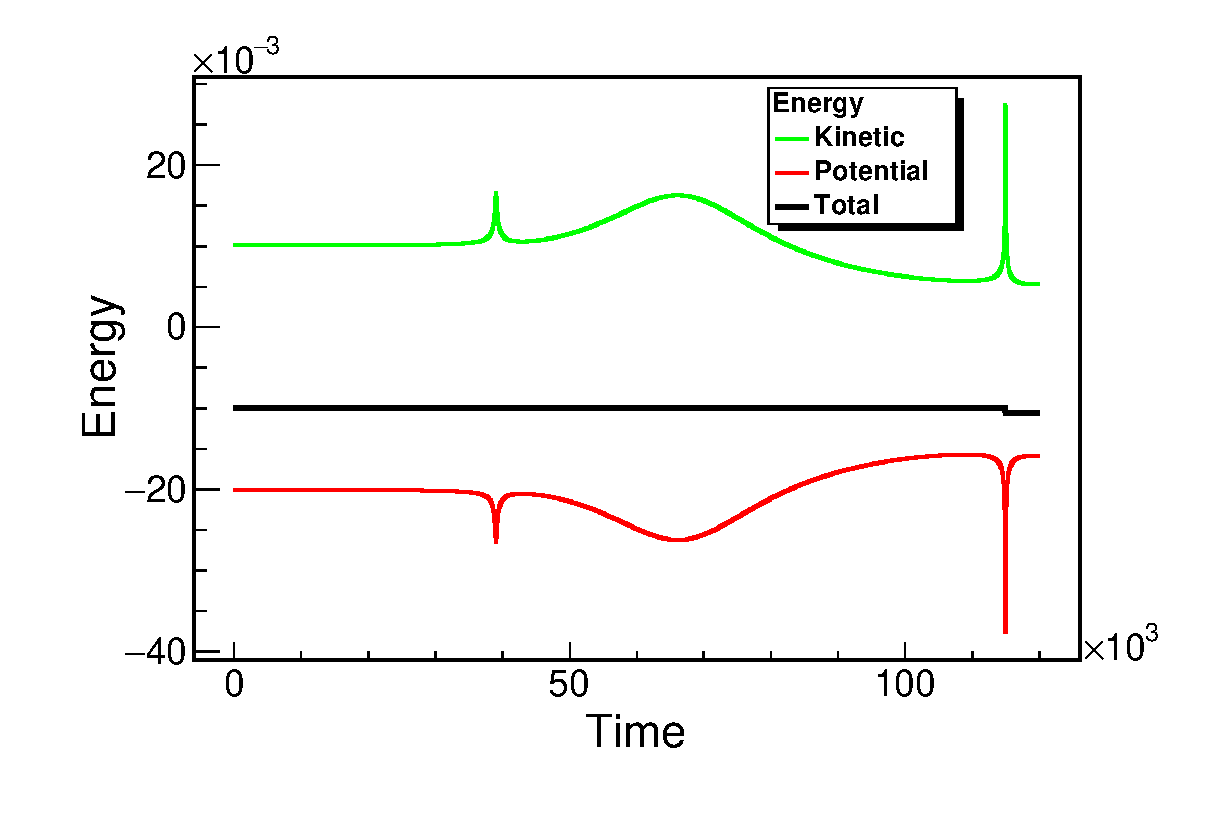
\includegraphics[width=0.5\textwidth]{figures/3ee.eps}}\\
\hfill
  \caption{\label{fig3} Plots for Part 3. Energy conservation is improved via the reduction in step size.}
\end{figure}
With an improved predictor-corrector algorithm, for example a trapezoid correction, would greatly enhance the integration convergence.
\clearpage
\subsection{Part 4}
The gravitational assist simulation is set up with the initial rocket conditions,
\begin{align*}
v_x &= -8.0 \\
v_y &= 1.225.
\end{align*}
This set of initial conditions ensures the rocket slingshots off Venus rather than the much more massive sun. Plots of the trajectories of the Earth (red), Venus (black), and the rocket (blue) show the rocket's liftoff from near Earth, it's pass around venus and the ``sling shot'' effect in Fig. \ref{fig4}.
\begin{figure}[h]
  \centering
  \subfloat[][]{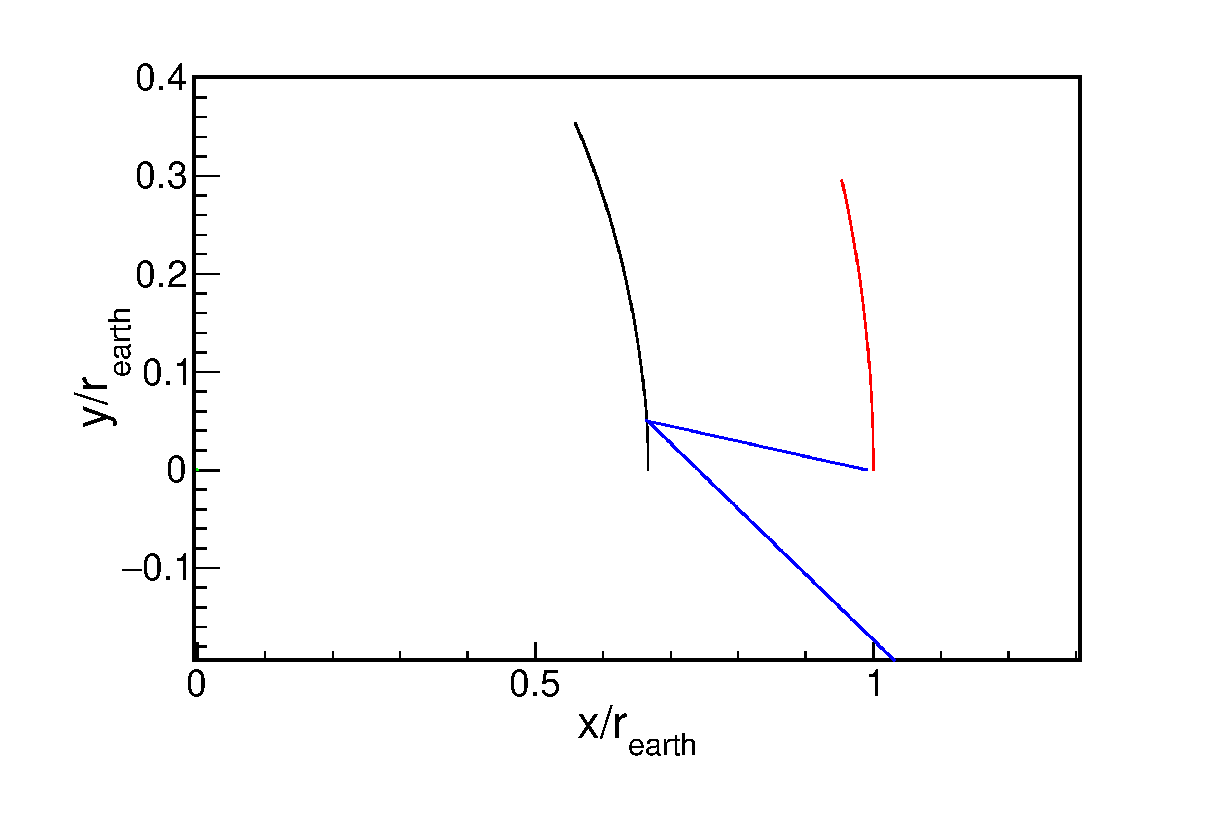
\includegraphics[width=0.5\textwidth]{figures/4r.eps}}
  \subfloat[][]{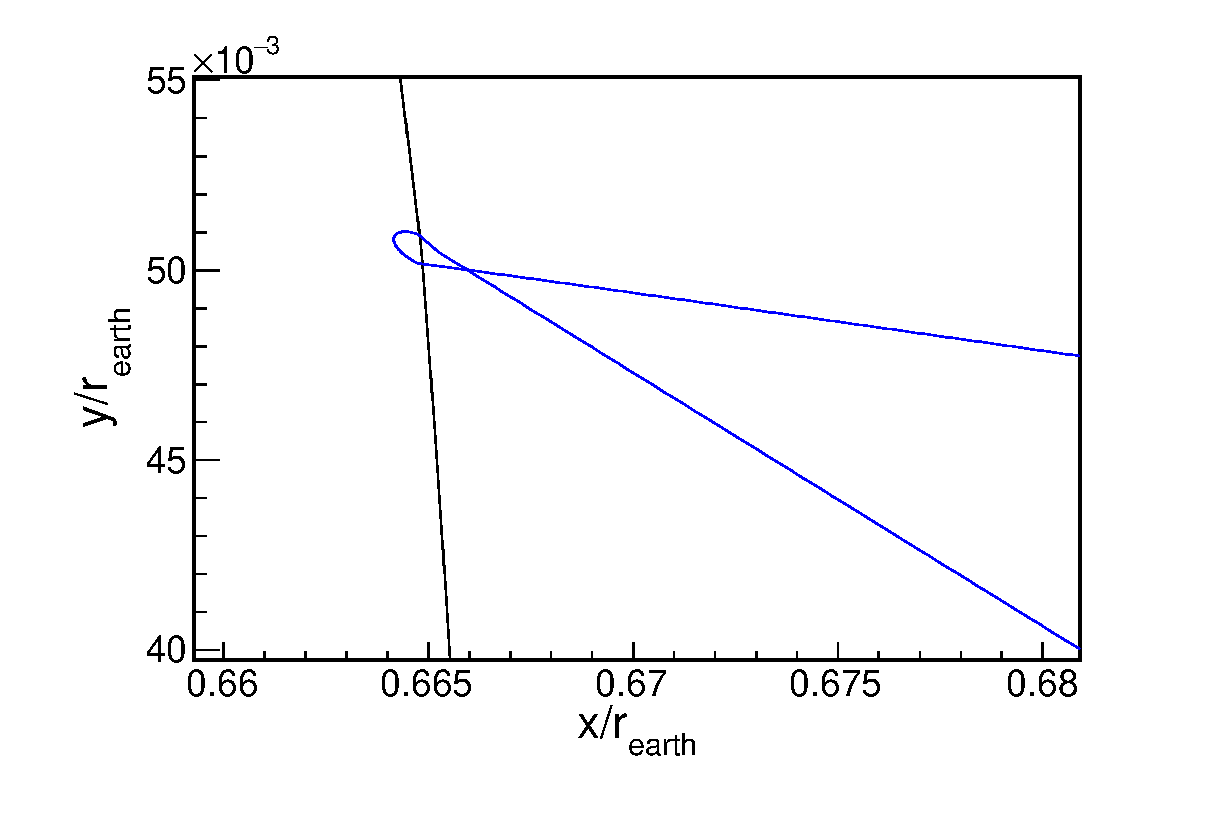
\includegraphics[width=0.5\textwidth]{figures/4r2.eps}}\\
\hfill
  \caption{\label{fig4} Plots for Part 4. The left pane shows the x-y positions of the three objects. The right pane is a close of the Venus-rocket interaction.}
\end{figure}
\clearpage
\section{Problem 2 - Liquid Argon}
The Lennard Jones potential is simulated for a gas of $N_p$ particles, in this case Liquid Argon, over $N_s$ time steps. The simulation was written in C++ with the aid of CERN's ROOT and the open source Boost C++ libraries. A summary of the code is as follows,
\begin{enumerate}
\item Execute main program \verb|develop| which either creates a \verb|LArgon| object from scratch, or reads an existing one out of the \verb|output/out.root| file. The main program \verb|develop| takes two option flags \verb|-r| for starting a new simulation or \verb|-c| to continue from an existing simulation and add molecular dynamics steps. \verb|develop -h| lists the command sequence.
\item The \verb|develop| program sets up the simulation on a \verb|LArgon| object by defining a number of private variables such as number of particles, steps, stepwise position, velocity, force, temperature, kinetic, potential energy, and a ``virial'' calculation.
\item The initial particle position is set on a lattice, and it's initial velocity distribution is generated uniformly on an interval with the \verb|boost::random::mt19937| generator with seed set via \verb|std::time(0)|. The center of mass velocity is set to zero and then scaled to the initial temperature.
\item The system is evolved for specified {\bf number of steps}, {\bf initial density}, {\bf number of particles}, and {\bf initial temperature} via the Velocity-Verlet algorithm with {\it periodic boundary conditions} and the {\it method of closest image}.
\item The final simulation completes and the object is stored in a ROOT file for inspection by \verb|mac/reader.py|. The simulation can also be further developed.
\end{enumerate}
To prove that the simulation works as expected, I ran the program with the following initial conditions:
\begin{itemize}
\item $N_P = 1000$ \# of particles. 
\item $N_s = 1000$ \# of steps.
\item $T_i = 2.0$ initial temperature.
\item $\rho = 1.0$ initial density.
\end{itemize}
The following initial position of the particles are shown in Fig. \ref{fig5}.
\begin{figure}[]
  \captionsetup[subfigure]{labelformat=empty}
  \centering
  \subfloat[][]{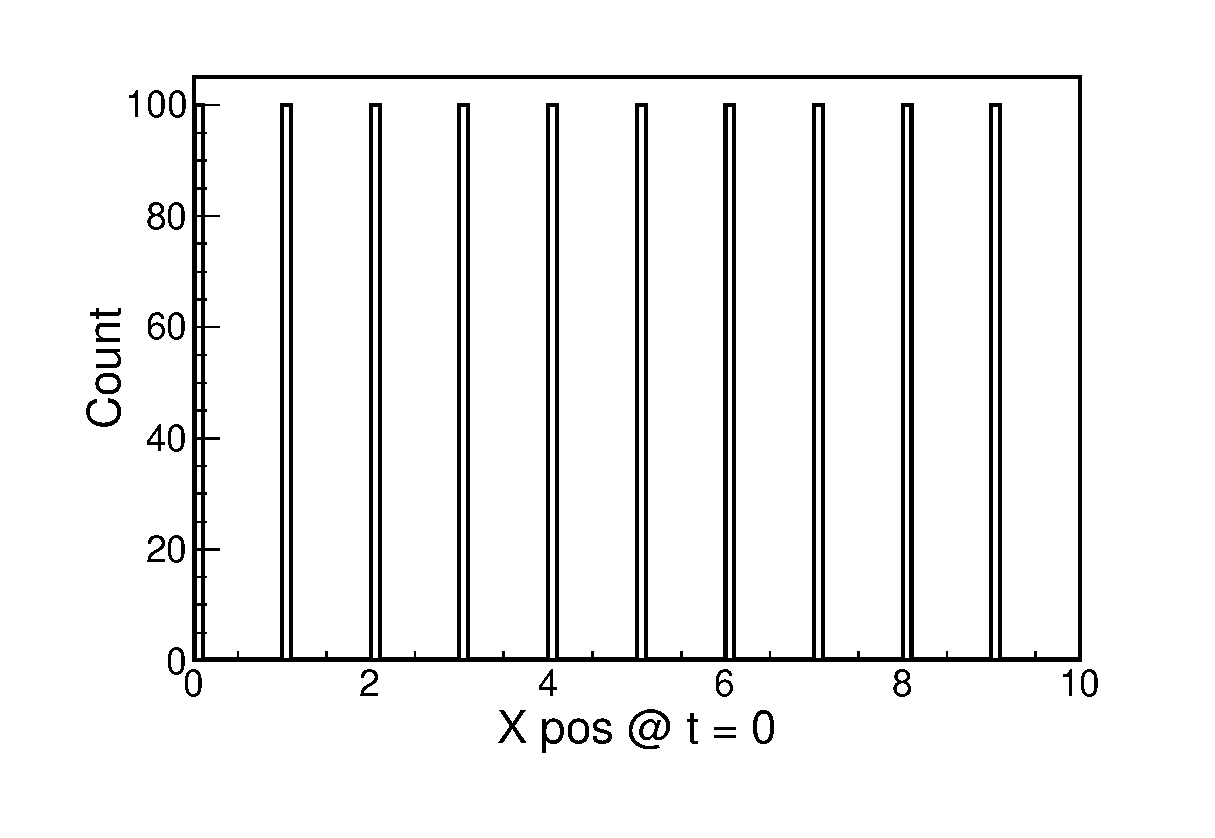
\includegraphics[width=0.5\textwidth]{figures/xpos_0.eps}}
  \subfloat[][]{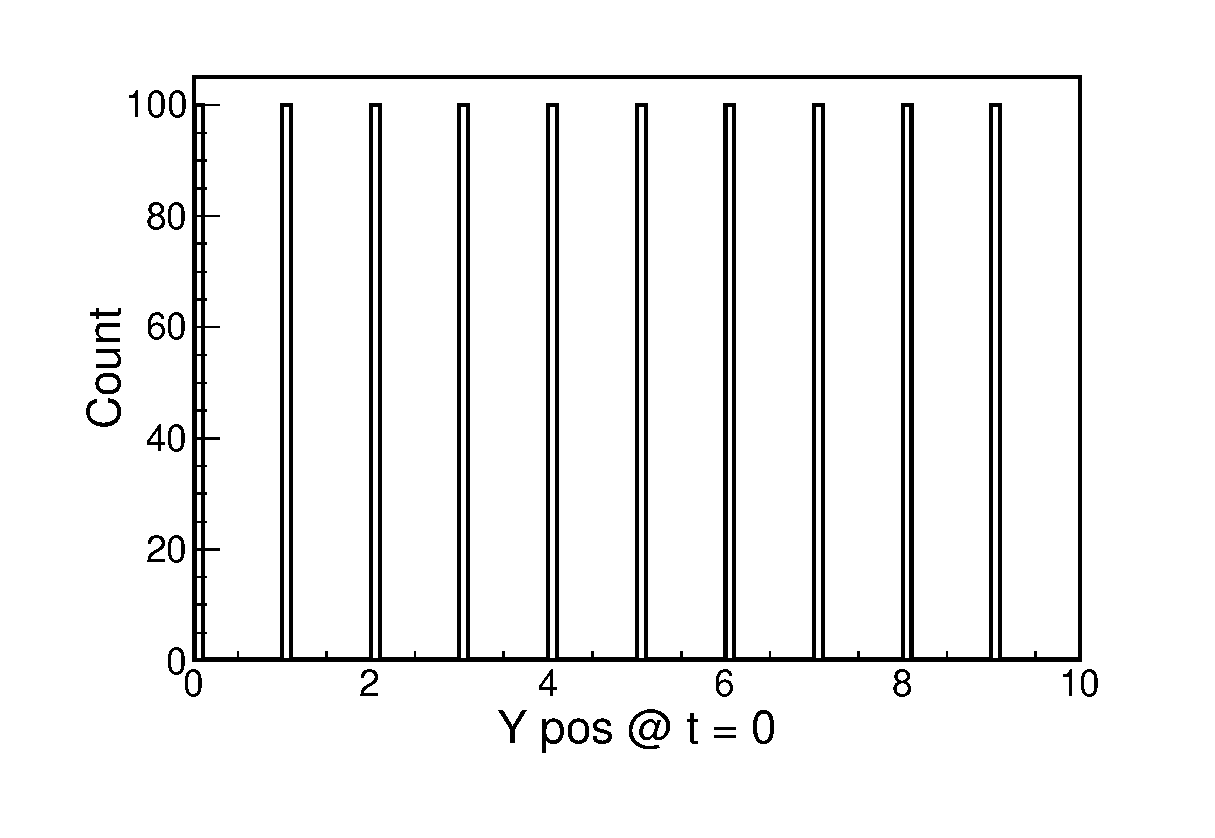
\includegraphics[width=0.5\textwidth]{figures/ypos_0.eps}}\\
  \subfloat[][]{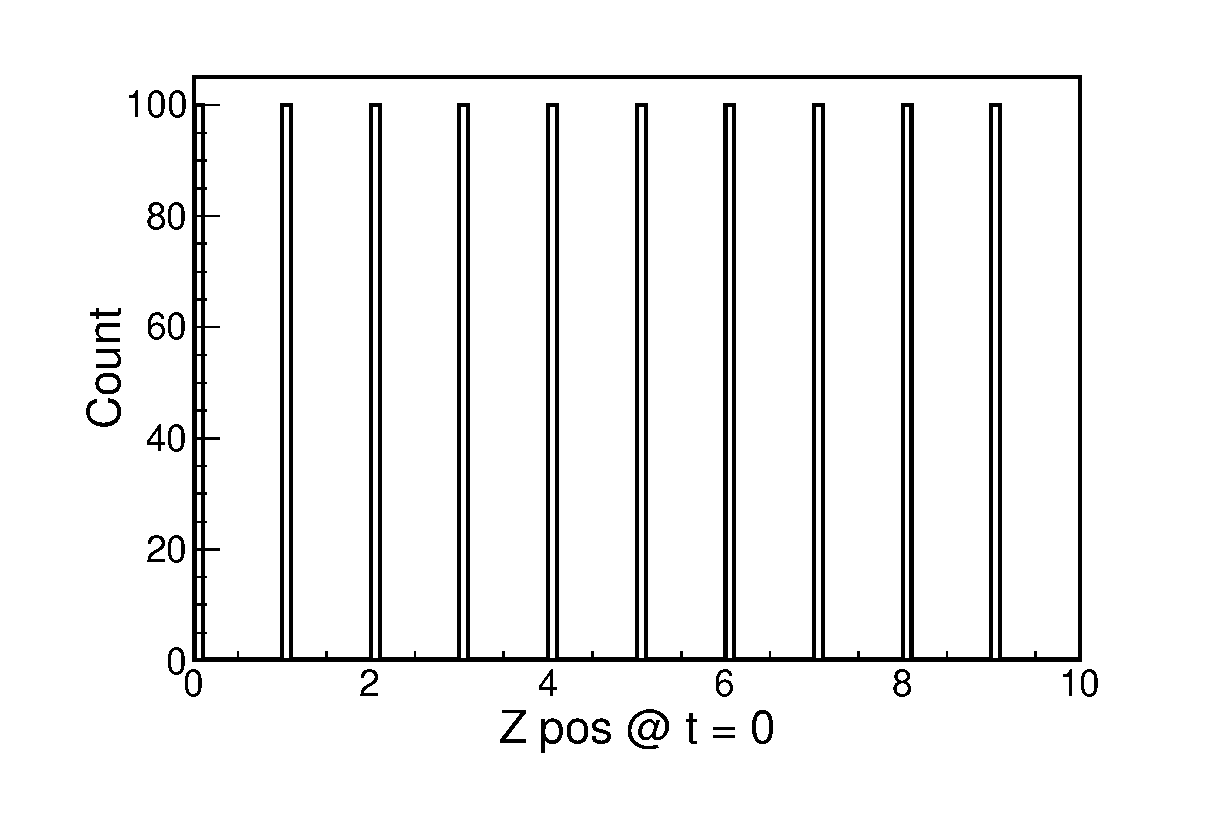
\includegraphics[width=0.5\textwidth]{figures/zpos_0.eps}}
\hfill
  \caption{\label{fig5} Histograms of initial positions of particles in X, Y, and Z directions.}
\end{figure}
Particles are spaced out based on requested density and number of particles. First, particles are placed maximally apart on the corners of a standard cubic lattice and then backfilled on the sites of a face-centered cubic until all the particles are placed in the box. If the number of particles is too high for the specified density and exceed particle separation larger than required on an fcc, the density and particle number are rejected by the program. Fig. \ref{fig6} shows the 1000 particles on the cubic lattice. Fig. \ref{fig7} shows the initial velocity distribution. After the simulation is evolved, the velocity distribution evolves to the expected Maxwell distribution as shown in Fig. \ref{fig8} and Fig. \ref{fig9}. The energy distribution if shown in Fig. \ref{fig10}. The system thermalizes relatively quickly, on the order of 40 steps. The simulation obeys time reversal. At step 250 all of the particle velocities are flipped in sign and the system evolves back to the initial state. This feature is shown in the temperature spectrum in Fig. \ref{fig11}. Code is implemented to determine the instantaneous pressure of the system by keeping track of the so called ``virial'' of the system, 
\begin{align*}
\text{virial} = \sum_i\sum_{i\neq j}r_{ij}F_{ij},
\end{align*}
which can be mapped to the pressure using the standard formula. For temperature $T\approx1.1$ at a density of $\rho=0.75$ the average ``compressibility''' was $\beta P/\rho \approx 0.88$ in near agreement with Verlet's paper. I was able to reduced the temperature by scaling all the velocities every hundred steps or so as shown in Fig. \ref{fig11}.
\begin{figure}[]
  \captionsetup[subfigure]{labelformat=empty}
\centering
  \subfloat[][]{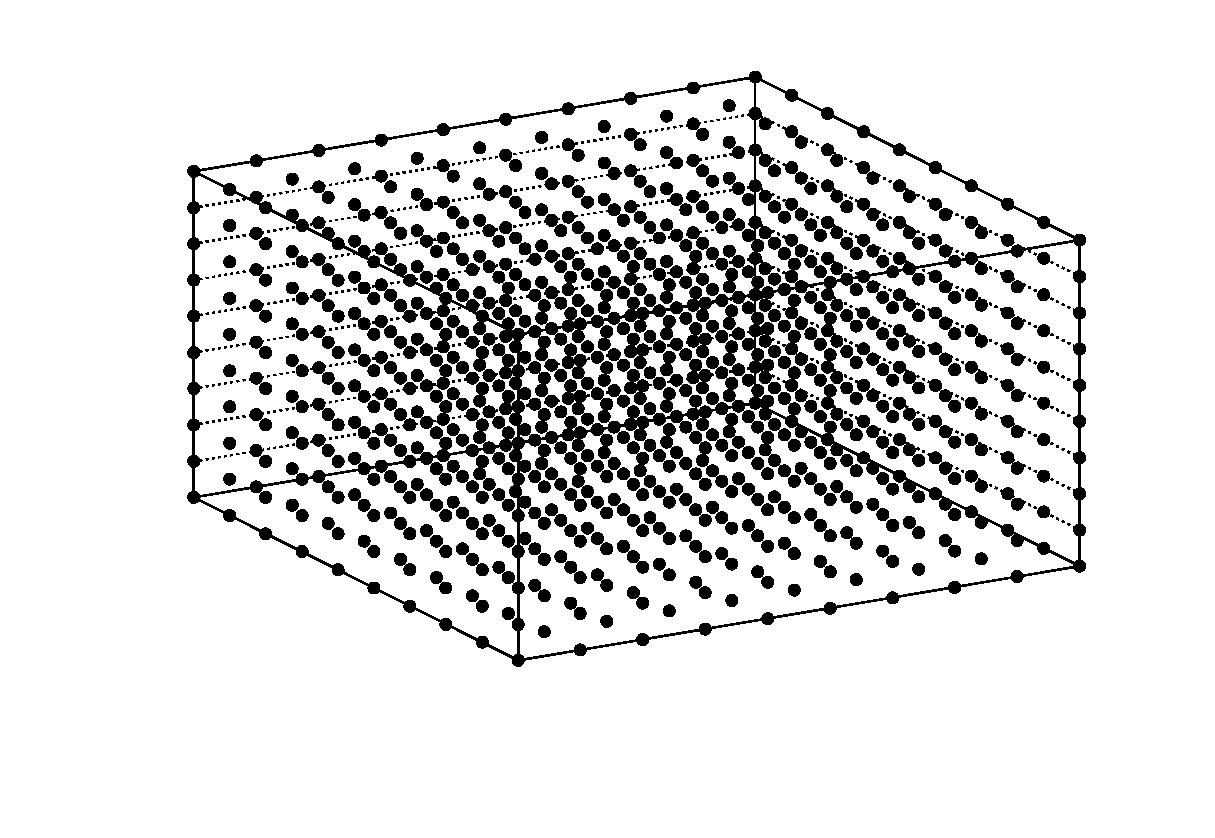
\includegraphics[width=0.5\textwidth]{figures/lattice_0.eps}}
  \subfloat[][]{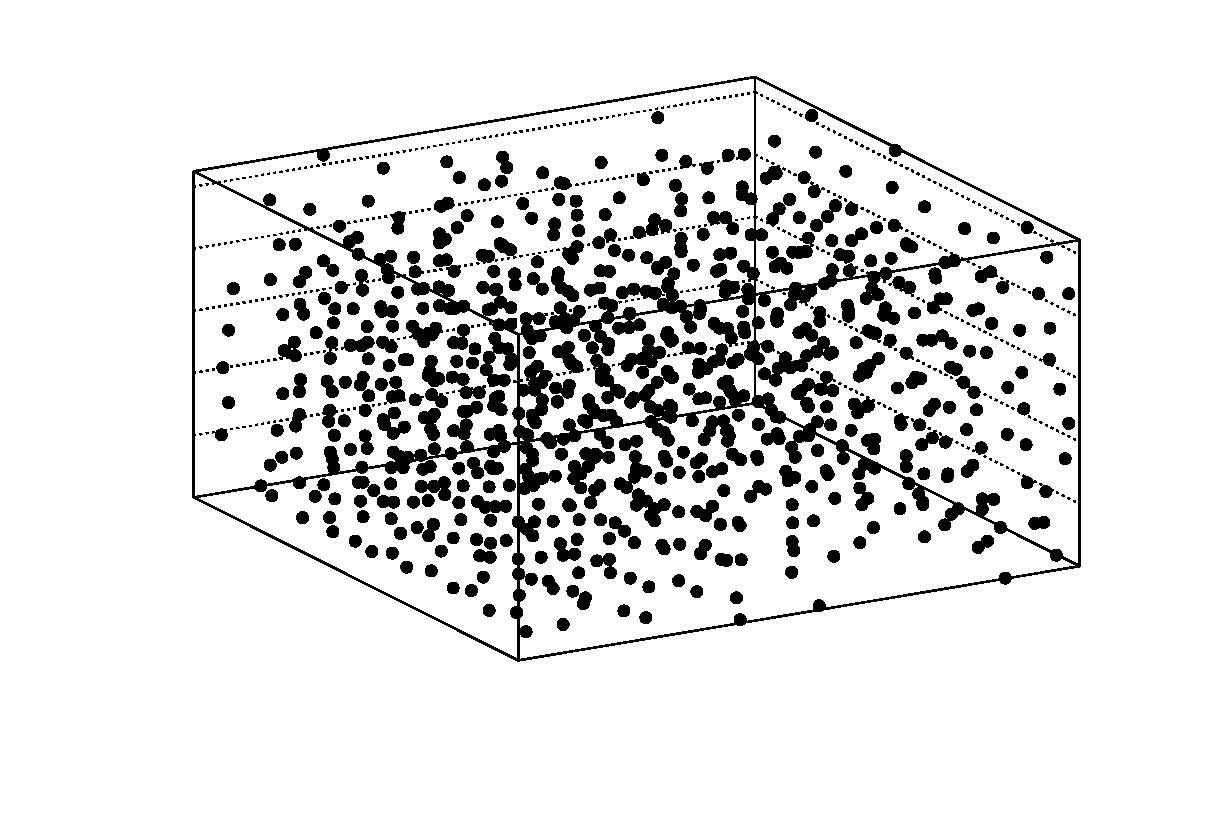
\includegraphics[width=0.5\textwidth]{figures/temp_thermal.eps}}
\caption{\label{fig6} 1000 particles on the lattice at $t=0$ and after thermalization.}
\end{figure}
\begin{figure}[]
  \captionsetup[subfigure]{labelformat=empty}
  \centering
  \subfloat[][]{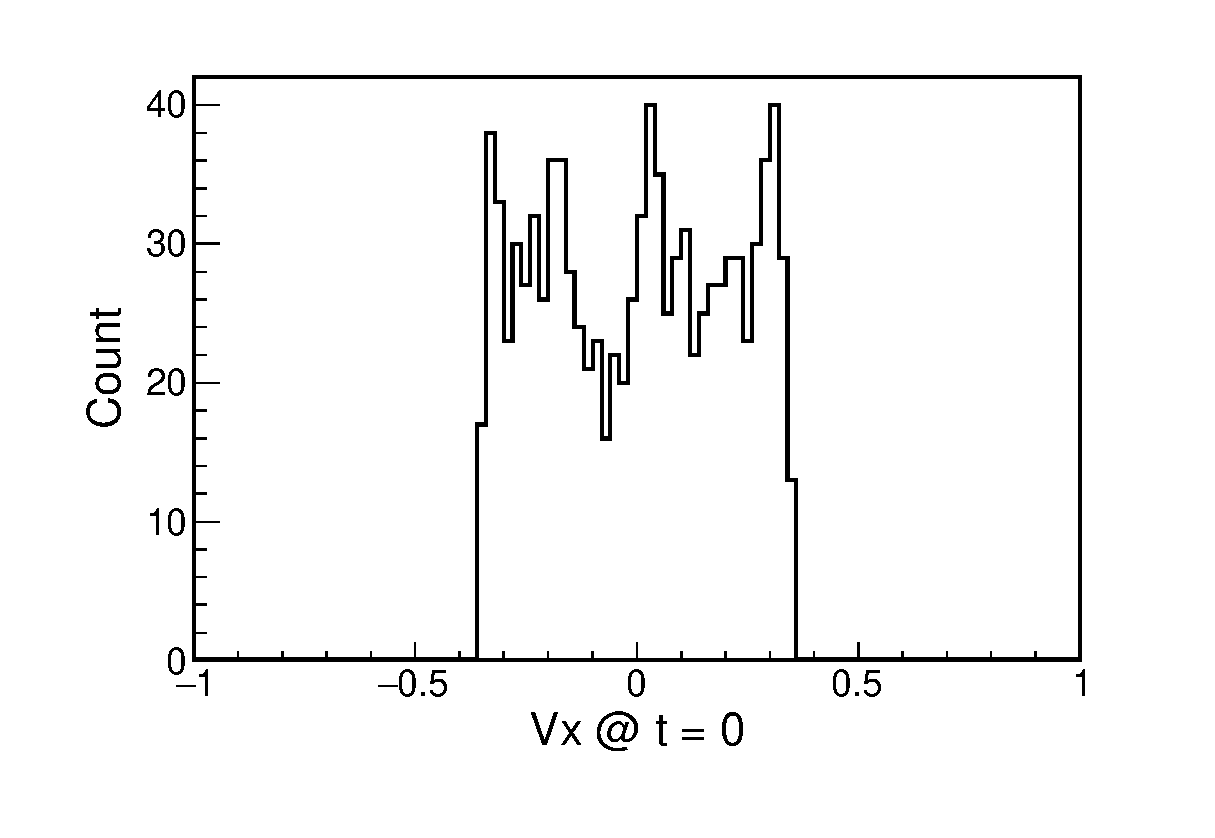
\includegraphics[width=0.5\textwidth]{figures/vx_0.eps}}
  \subfloat[][]{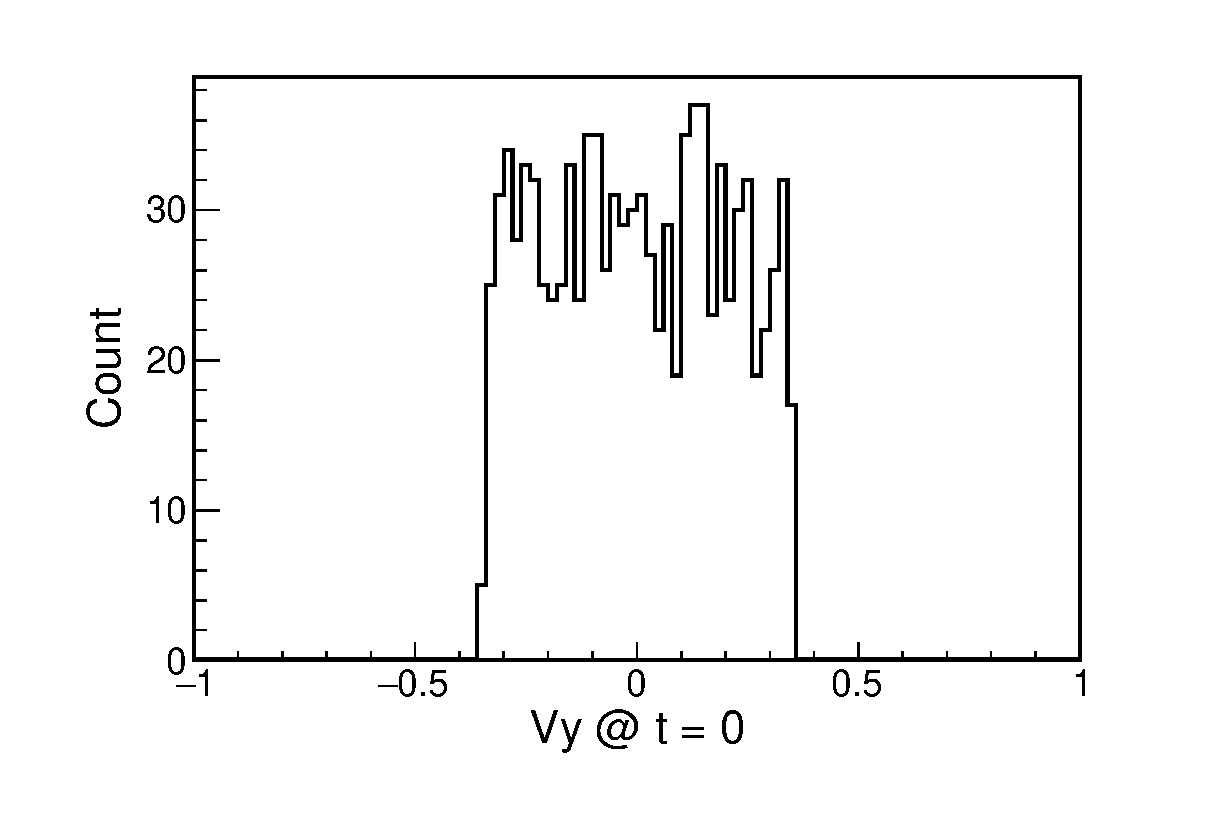
\includegraphics[width=0.5\textwidth]{figures/vy_0.eps}}\\
  \subfloat[][]{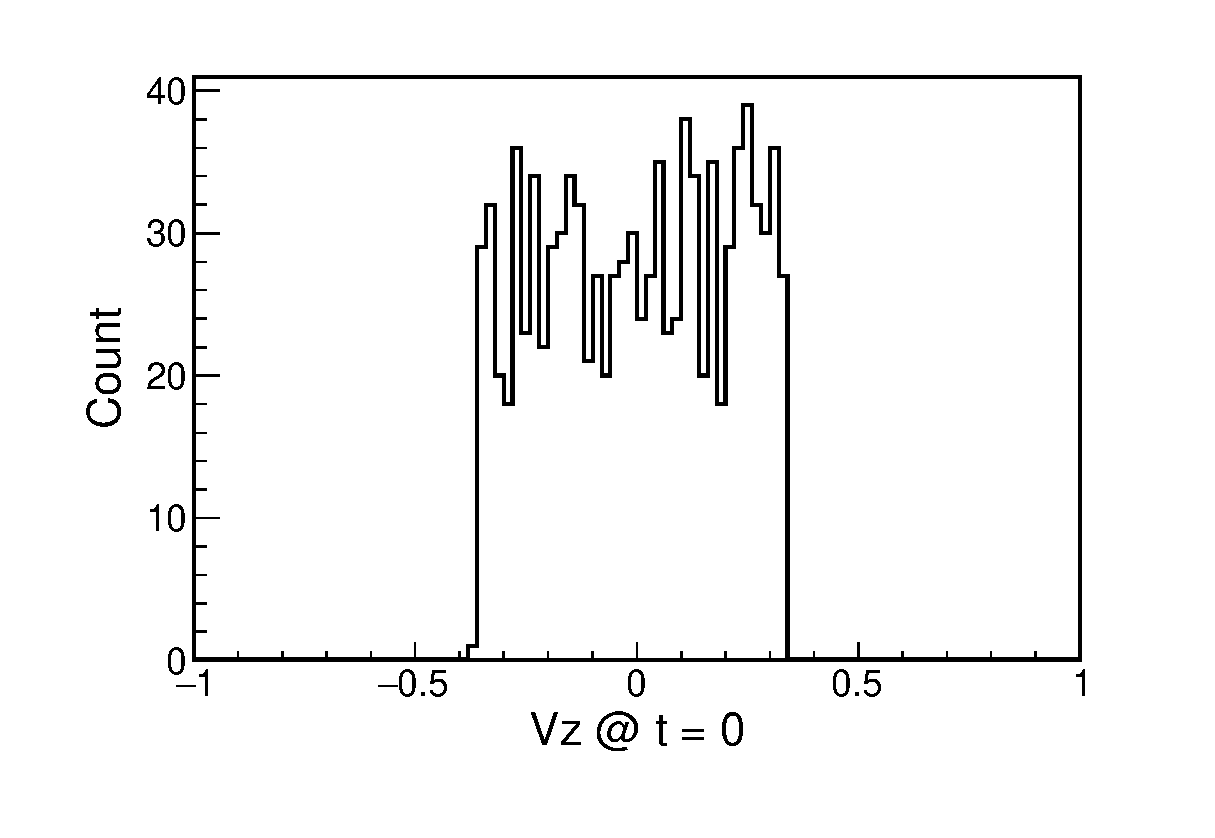
\includegraphics[width=0.5\textwidth]{figures/vz_0.eps}}
\hfill
  \caption{\label{fig7} Histograms of initial velocity of particles in X, Y, and Z directions.}
\end{figure}
\begin{figure}[]
  \captionsetup[subfigure]{labelformat=empty}
  \centering
  \subfloat[][]{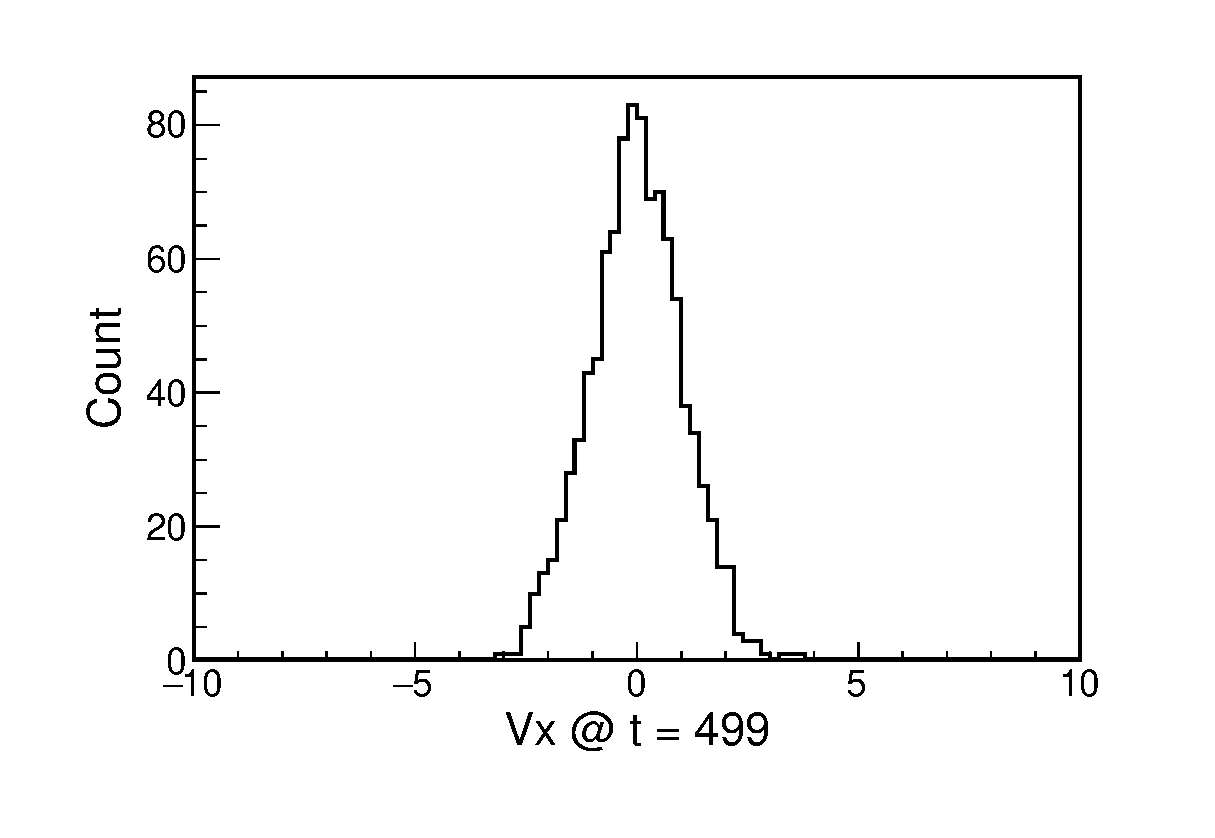
\includegraphics[width=0.5\textwidth]{figures/vx_499.eps}}
  \subfloat[][]{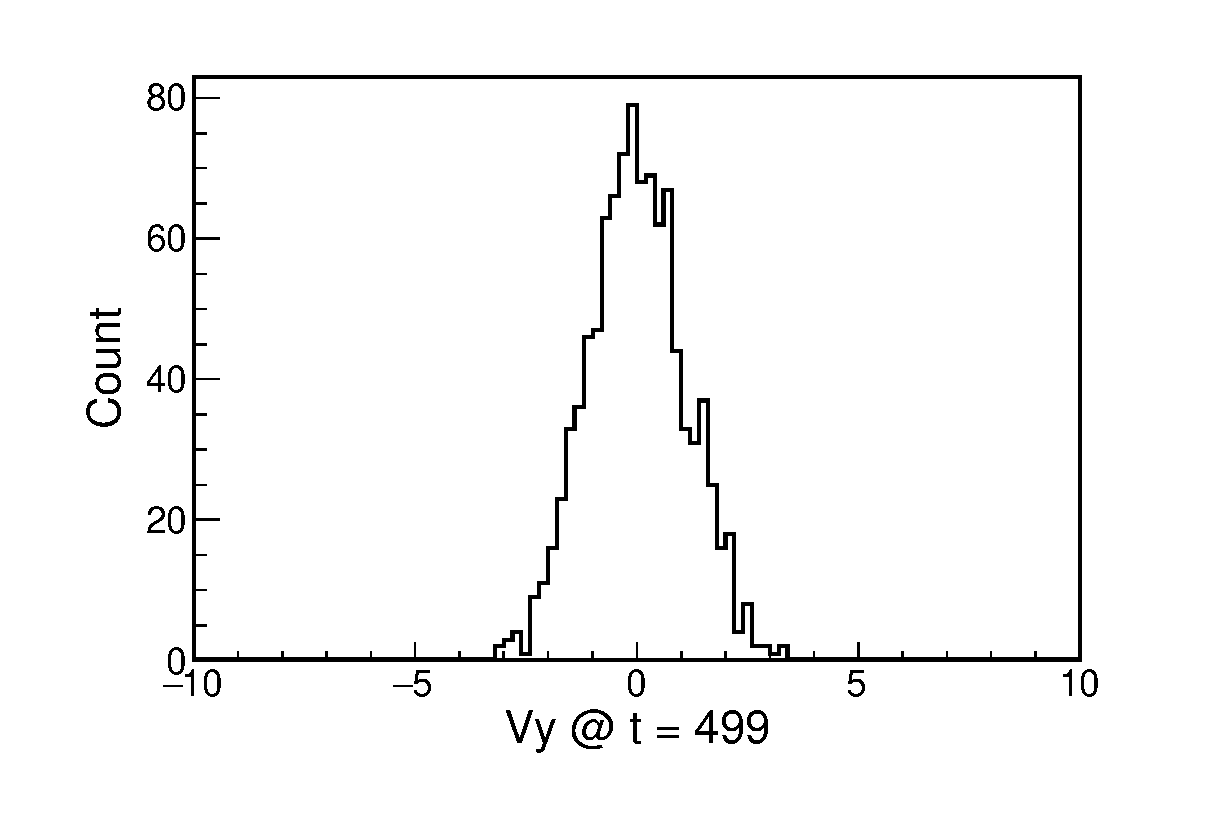
\includegraphics[width=0.5\textwidth]{figures/vy_499.eps}}\\
  \subfloat[][]{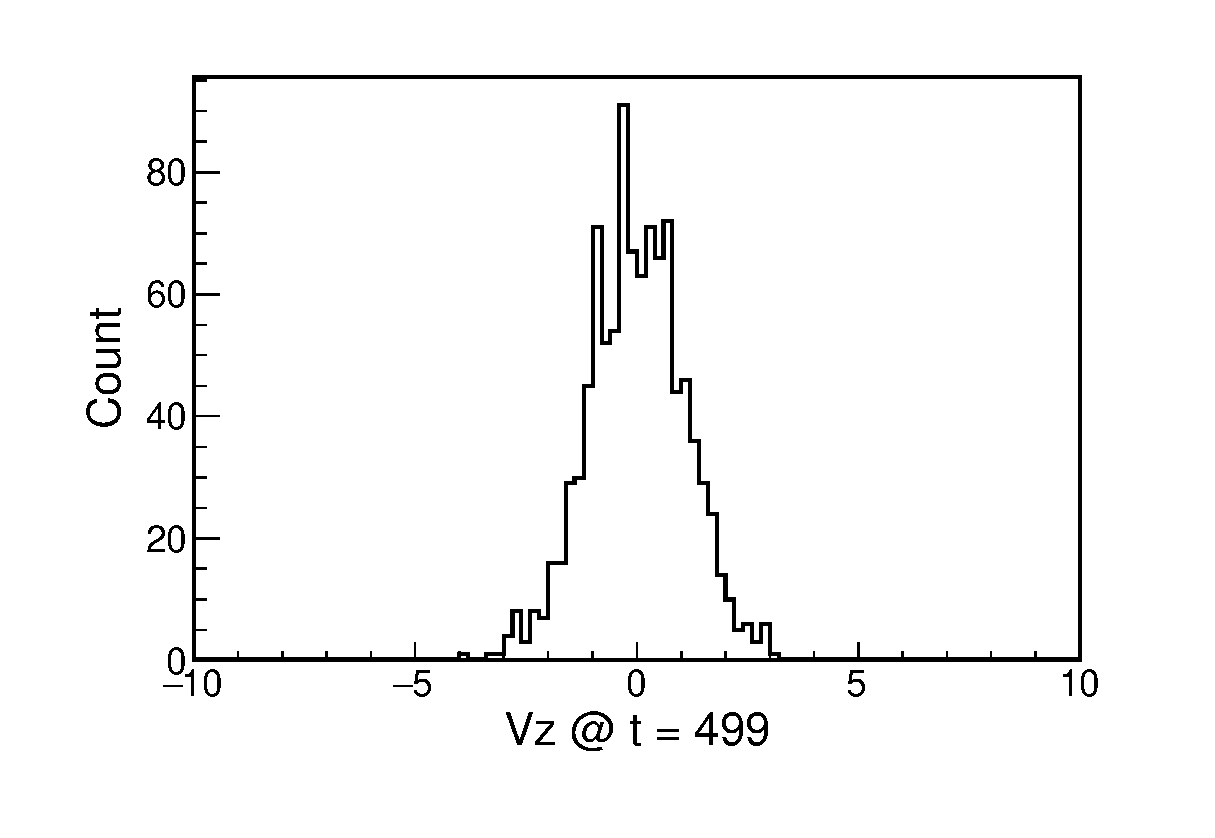
\includegraphics[width=0.5\textwidth]{figures/vz_499.eps}}
 \hfill
  \caption{\label{fig8} Histograms of final velocity of particles in X, Y, and Z directions.}
\end{figure}
\begin{figure}[]
  \centering
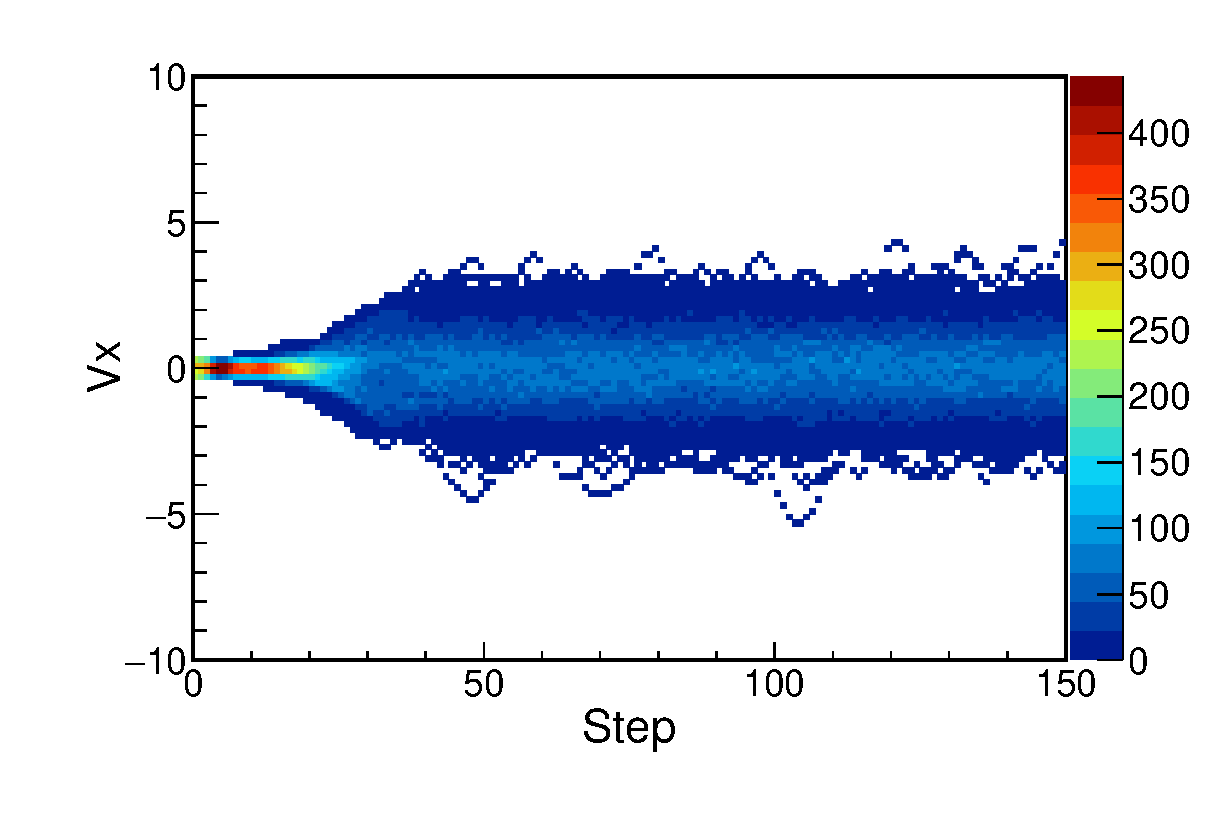
\includegraphics[width=0.6\textwidth]{figures/vx_step.eps}
\hfill
\caption{\label{fig9} 2D histogram showing the time evolution of the velocity distribution in the x direction. The Z axis color is the number of particles in each bin. As time progresses the velocities of particles spread out as the system thermalizes.}
\end{figure}
\begin{figure}[]
  \captionsetup[subfigure]{labelformat=empty}
  \centering
  \subfloat[][]{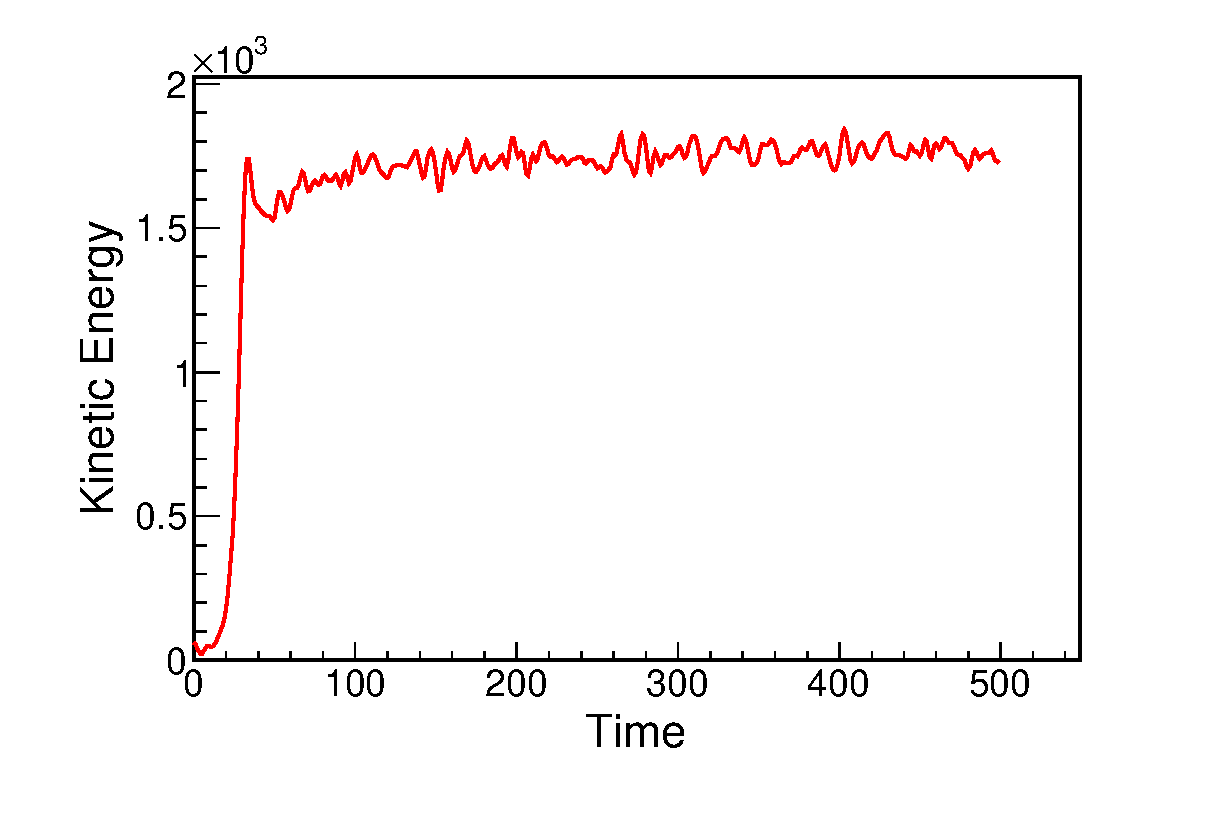
\includegraphics[width=0.5\textwidth]{figures/kinetic.eps}}
  \subfloat[][]{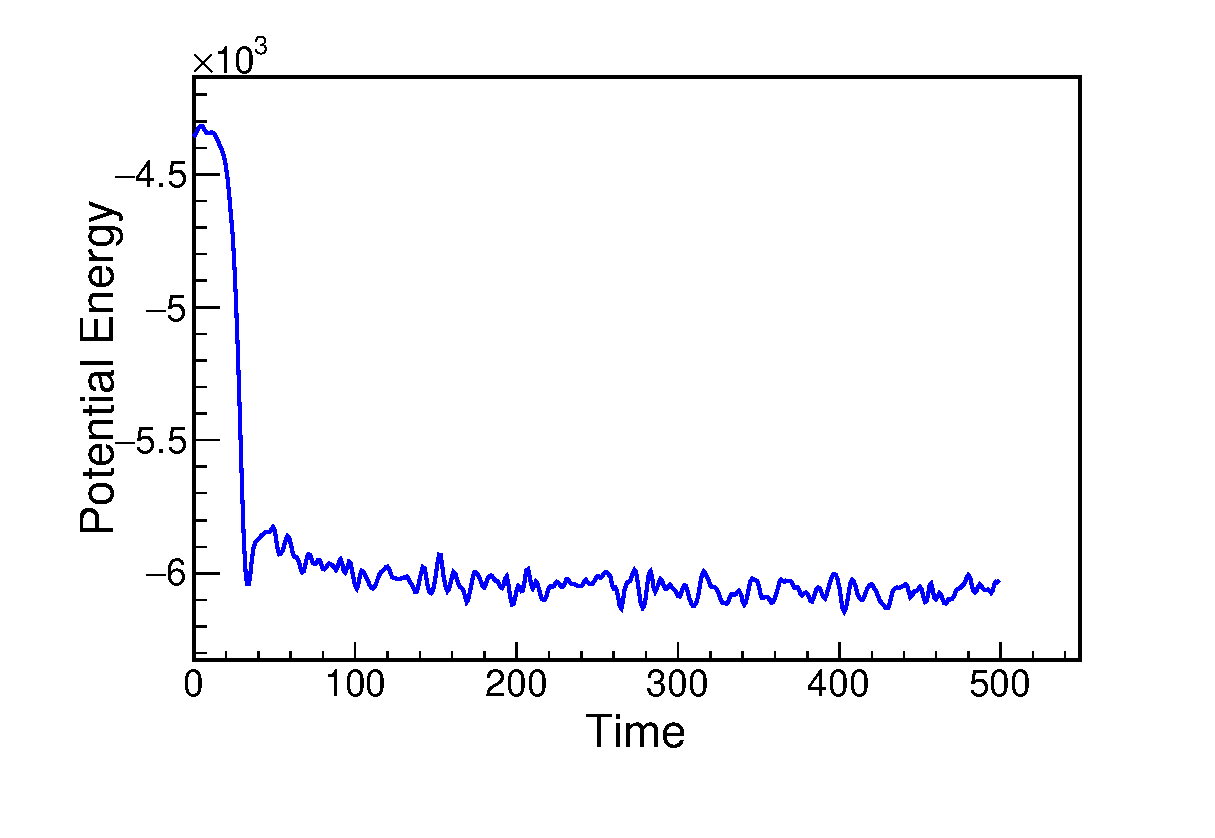
\includegraphics[width=0.5\textwidth]{figures/potential.eps}}\\
  \subfloat[][]{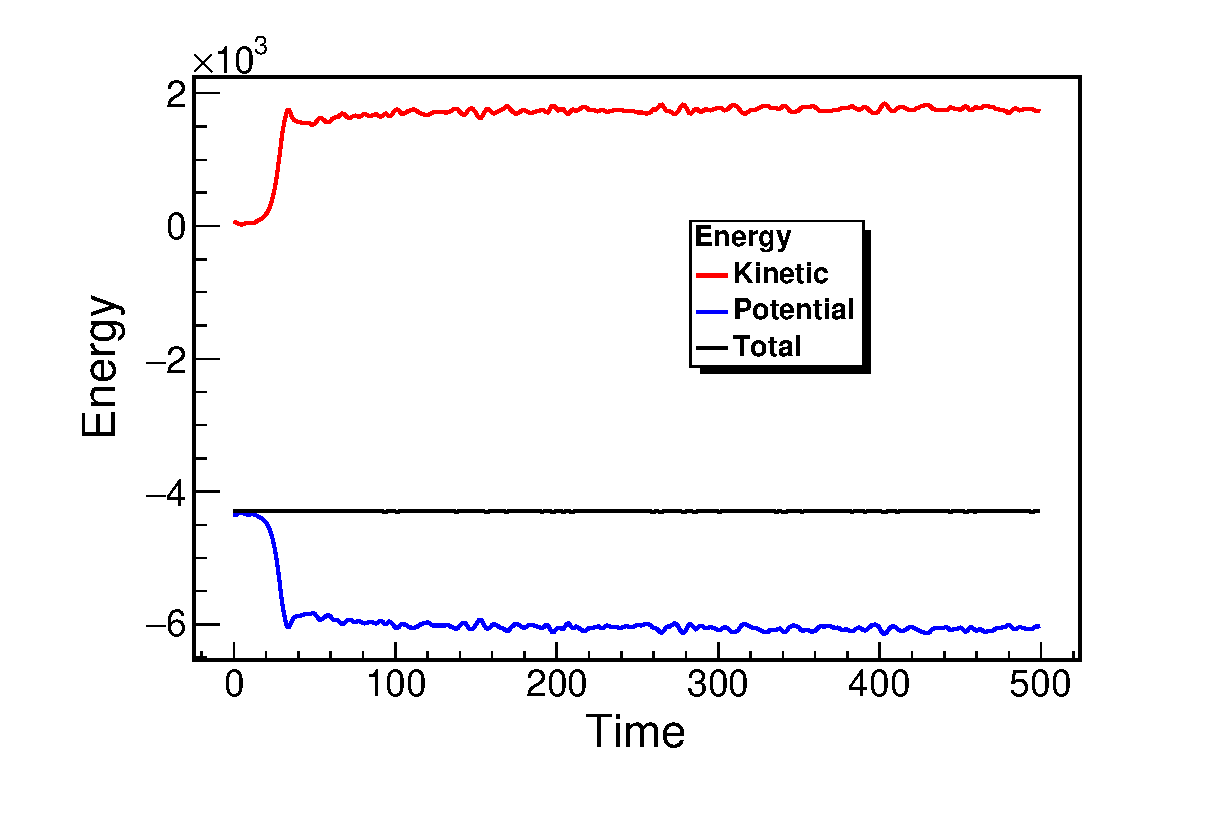
\includegraphics[width=0.5\textwidth]{figures/energy_all.eps}}
  \subfloat[][]{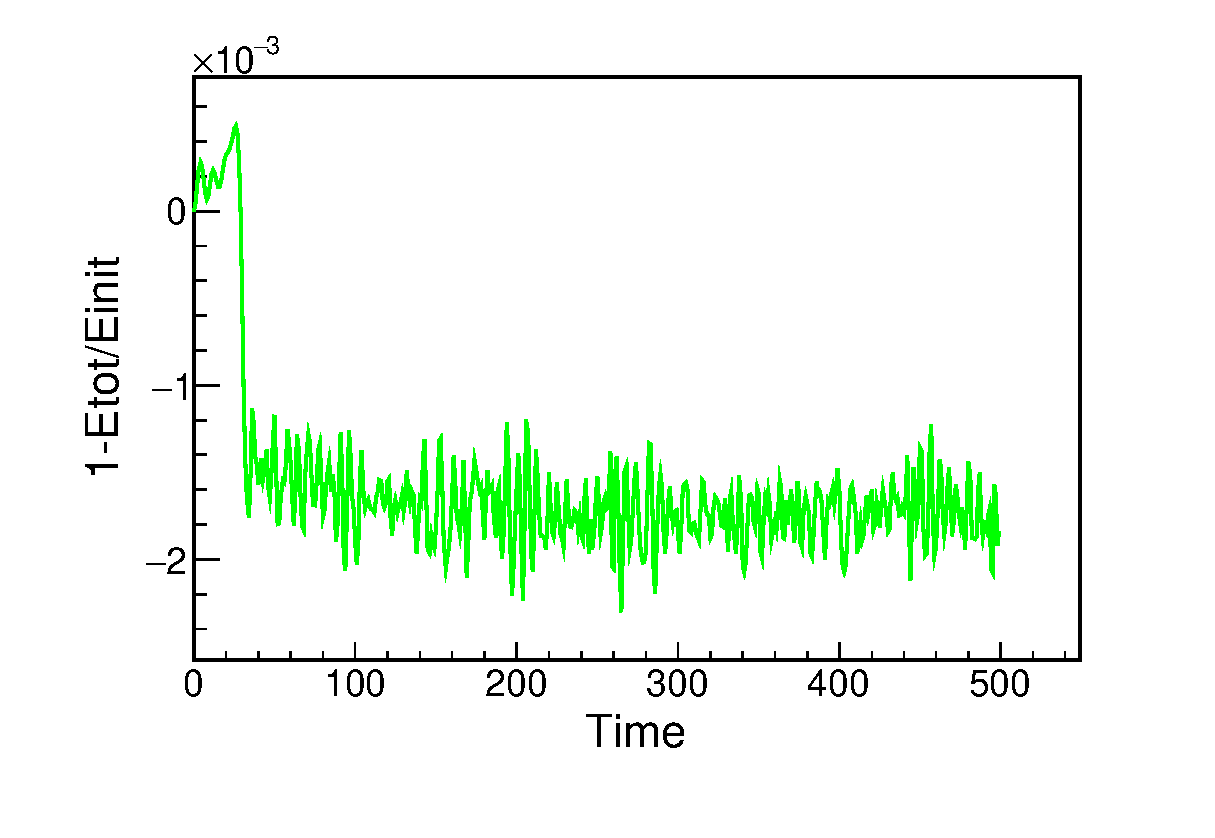
\includegraphics[width=0.5\textwidth]{figures/e_diff.eps}}
  \hfill
  \caption{\label{fig10} Graphs of instantaneous kinetic, potential, and total energy. The bottom right pane shows the deviation of the total energy from $t=0$.}
\end{figure}
\begin{figure}
  \captionsetup[subfigure]{labelformat=empty} 
  \centering
  \subfloat[][]{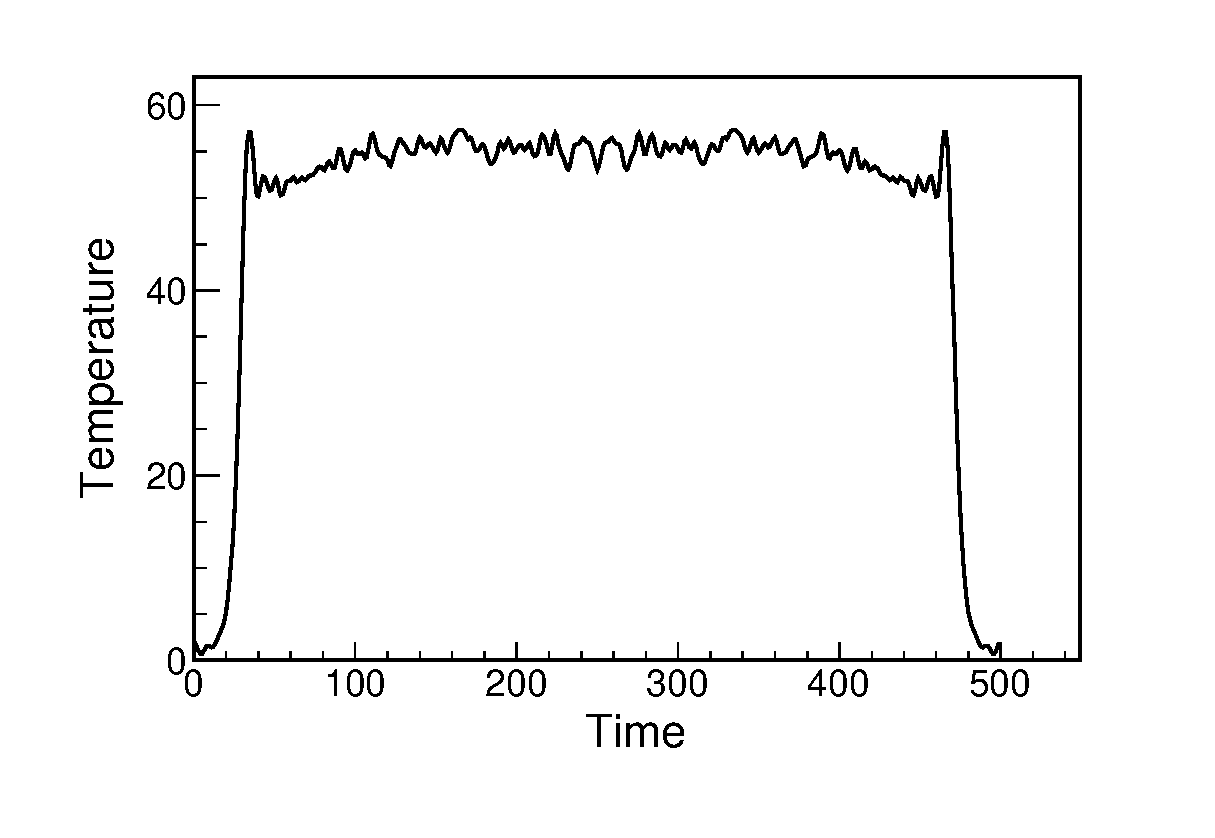
\includegraphics[width=0.5\textwidth]{figures/temp.eps}}
  \subfloat[][]{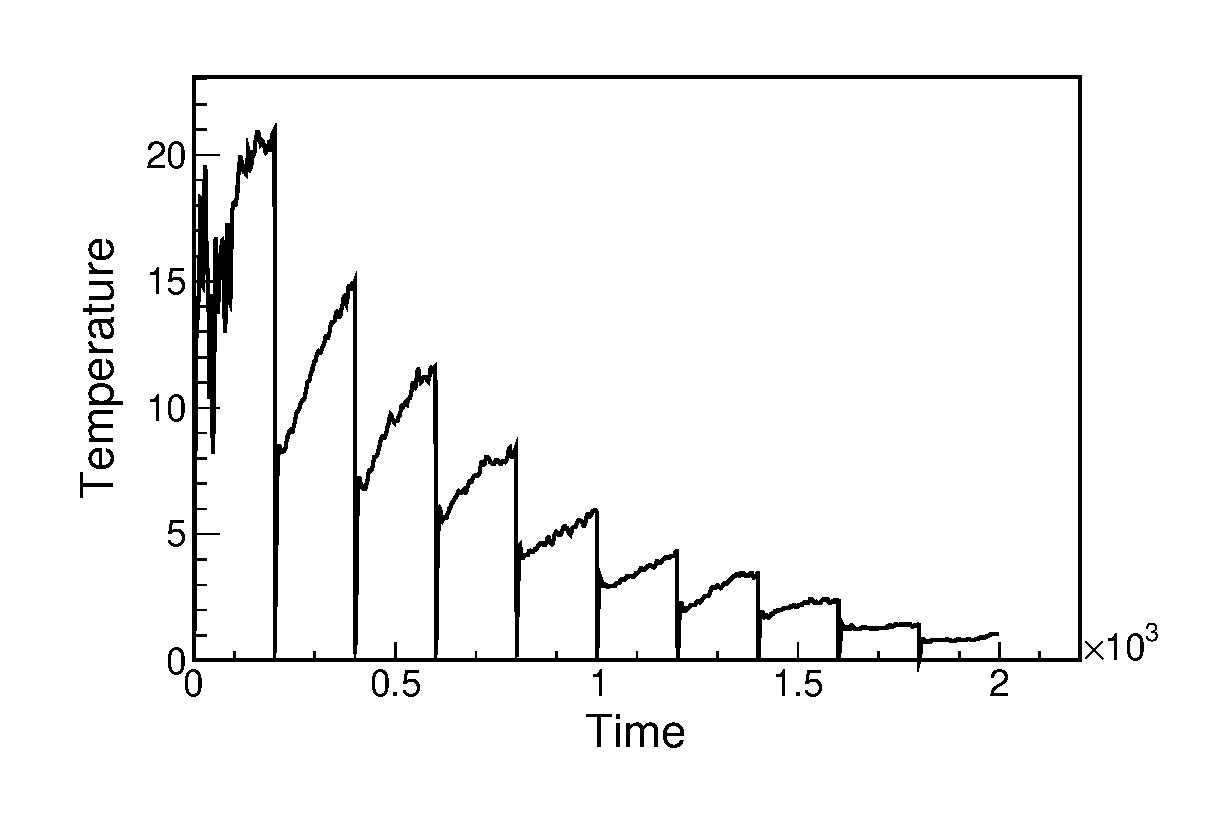
\includegraphics[width=0.5\textwidth]{figures/temp_reg.eps}}
\hfill
\caption{\label{fig11} Temperature spectra. In the top left pane, the system is reversed at $t=250$ and evolved back to its initial condition, demonstrating reversibility. The right pane shows temperature reduction over 2000 steps via velocity scaling.}
\end{figure}
\end{document}
